\documentclass[12pt,twoside,a4paper]{article}

\usepackage[english]{babel}
\usepackage{blindtext}

\usepackage[margin=1in]{geometry}
\usepackage{lmodern}
\renewcommand\familydefault{lmss} % lmdh

\usepackage{microtype}

\usepackage{graphicx} % including external figures
\usepackage{wrapfig} % wrapping text around figures
\usepackage{enumitem} % enumerating/listing points
\usepackage{fancyhdr} % header/footer
\usepackage{amsmath} % maths
\usepackage{hyperref} % hyperlinks, cross-referencing

\usepackage{enumitem} % enumerating points (named itemize)

\hypersetup{
  colorlinks=true,
  linkcolor=red,
  citecolor=blue,
  urlcolor=blue
}

\usepackage{fancyhdr}
\pagestyle{fancy} % use fancy header instead of default header
\fancyhf{} % clear existing header formatting
\renewcommand{\headrulewidth}{0.5pt} % header-line width
\renewcommand{\footrulewidth}{0.5pt} % footer-line width
\fancyhead[LE,RO]{Nikhil Vidhani} % name on left-side on even pages and right-side on odd pages
\fancyhead[LO,RE]{Intro to \LaTeX} % title on left-side on odd pages and right-side on even pages
\fancyfoot[C]{Page: \thepage} % centred footer on all pages
\fancyfoot[L]{Section: \thesection} % section number of left-side for all pages
\fancyfoot[R]{Article: 1} % article number of right-side for all pages



% \usepackage[singlespacing]{setspace}
\usepackage[onehalfspacing]{setspace}
% \usepackage[doublespacing]{setspace}


\usepackage{booktabs} % provides different line thicknesses to be used in tables like \toprule, \midrule, \bottomrule, \hline



% custom commands
\newcommand{\tableinfo}{
All independent variables are one month lagged variables. Definitions of all the variables appears in Appendix A2. All regression specifications have industry and year fixed effects. Standard errors are double clustered by firm and year-month. Statistical significance of 10\%, 5\% and 1\% are indicated by *, ** and *** respectively.
}
\newcommand{\contact}[3]{
    Author is a final year PhD student at \href{#1}{Indian Institute of Management, Bangalore}. \emph{email}: \href{mailto:#2}{#2}. Phone: \href{tel:#3}{#3}
}



\usepackage{subcaption}



\usepackage{longtable}




\usepackage[natbibapa]{apacite}
\bibliographystyle{apacite}





\title{Introduction to \LaTeX}
\author{Nikhil Vidhani\thanks{\contact{https://sites.google.com/view/nikhilvidhani}{nikhil.vidhani16@iimb.ac.in}{+91-797-555-7296}}}


\begin{document}

\maketitle
\tableofcontents
\listoftables
\listoffigures

\newpage
\begin{abstract}
This document is prepared as a handy reference guide for the class \textbf{Introduction to \LaTeX}. Different topics covered in the class are organized in different sections. You should be able to use this as a template and write your own version of report, article or thesis. At some places I use \verb|blindtext| which is fancy word for \emph{gibberish}. It is used to show the formatting and look of the document. However in sections concerning line-breaks, special characters, math symbols and citations I use text that should be used by looking at the corresponding latex code.
\end{abstract}


\newpage
\section{List}
\begin{itemize}
	\item 1 Cup Spinach
	\item 1 Cup Frozen Blueberries
	\item 2 Bananas
	\item 1.5 Cups Almond Milk
	\item Powders
	% List within a list
	\begin{itemize}
		\item 1 Tbs PBJ
		\item 1 Tsp Amla Powder
		% List within a list within a list
		\begin{itemize}
		    \item 1 tsp sugar
		    \item 0.5 tsp salt
		\end{itemize}
	\end{itemize}
	\item six Dates
\end{itemize}



\section{Enumeration}
\begin{enumerate}[font=\bfseries]
	\item 1 Cup Spinach
	\item 1 Cup Frozen Blueberries
	\item 2 Bananas
	\item 1.5 Cups Almond Milk
	\item Powders
	\begin{enumerate}[font=\itshape]
		\item 1 Tbs PBJ
		\item 1 Tsp Amla Powder
		\begin{enumerate}
			\item 1 tsp sugar
			\item 0.5 tsp salt
		\end{enumerate}
	\end{enumerate}
	\item six Dates
\end{enumerate}


\section{Figure}
\begin{figure}[ht] % h:here, t: top, b: bottom (best-effort only)
\centering % to centre the figure
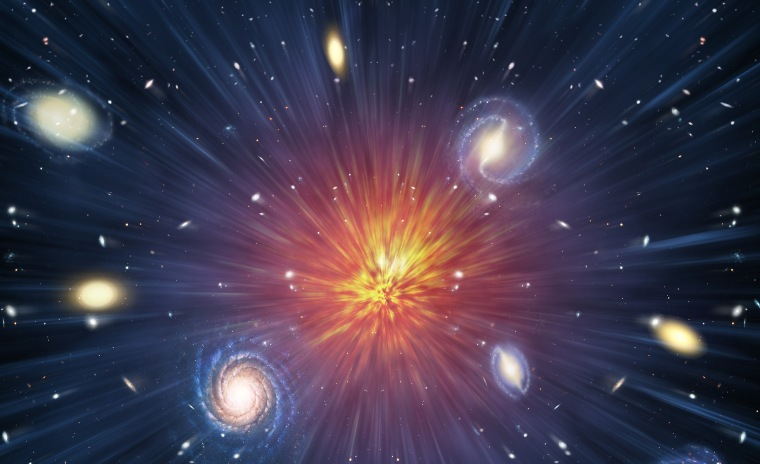
\includegraphics[width=4in]{universe.jpg}
\caption{This is a figure!}
% can be a pdf too. In fact, pdfs (vector graphics) are preferred for plots. Try playing with the width argument!
\end{figure}


\clearpage
\section{Wrapped Figure}
\blindtext[1]
\begin{wrapfigure}{r}{0.5\textwidth} % r: right, l: left, i: inside-edge, o: outside-edge. i and o are w.r.t. odd/even page. 
% Image width relative to text width
\centering % to centre the figure
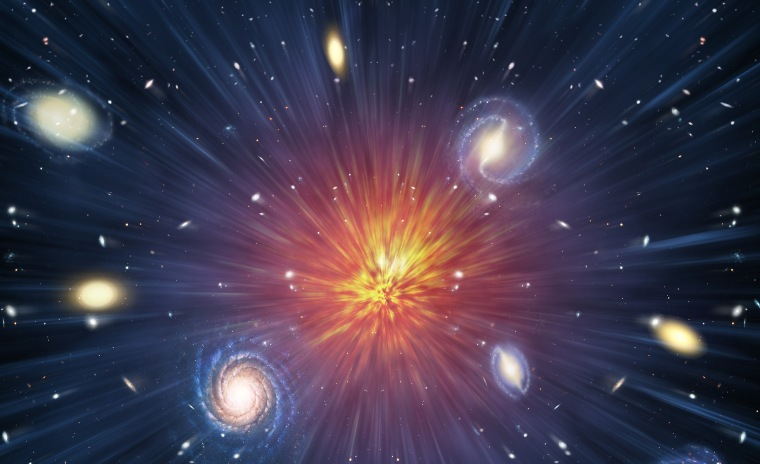
\includegraphics[width=\linewidth]{universe.jpg} % \linewidth changes in different environments (wrapfigure)
\caption{This is a wrapped figure!}
\end{wrapfigure}
\blindtext[1]




\section{Sub-sections}
Section body!
\subsection{Name of subsection}
Sub-section body!
\subsubsection{Name of subsubsection}
Sub-sub-section body!
\subsection*{Sub-section w/o a name}
Sub-section body!



\section{Line Breaks}
First-line of a section is not indented.
A simple carriage-return (enter) doesn't change anything.
To get a line-break enter two backslashes (\textbackslash\textbackslash) after the end of line.\\
This line appears after a line-break. Note that here also there is no-indent.\\\\
In fact, multiple line-breaks also do not create indent!
More space can be added by specifying amount.\\[20pt]
Lot of gap now!

Adding two carriage-returns (enters) means a change of paragraph. Here there will be indent.
You can use \textbackslash\texttt{noindent} to skip indentation.

\noindent No indent here! If you want no indentation in the entire document then use \textbackslash\texttt{usepackage\{parskip\}}





\section{Special Characters}
Latex has some special characters: `\{’, `\}’, `\#’, `\%', `\$', `\&', `\_' and, `\textbackslash'. To print them you must use a \textbackslash, i.e. \textbackslash\texttt{\{}, \textbackslash\texttt{\}}, \textbackslash\texttt{\#}, \textbackslash\texttt{\%}, \textbackslash\texttt{\$}, \textbackslash\texttt{\&} and, \textbackslash\texttt{\_}. For printing `\textbackslash' you have to use the command \textbackslash\texttt{textbackslash}

\noindent Alternatively, you could use \verb|\{| to print \{


\section{Tabbing}
A simple tabbed list. Think of it like a bare-bone table without lines.
\begin{tabbing}
\textbf{S.No.} \hspace{0.5in} \= \textbf{Name} \hspace{0.5in} \= \textbf{City} \hspace{0.5in} \= \textbf{Area} \\
1 \> Nikhil   \> Agra   \> Finance \\
2 \> Abhishek \> Ranchi \> Economics \\
3 \> Pranjal  \> Raipur \> Decision Sciences \\
\end{tabbing}



\section{Tabular}
\begin{tabular}{|  l  ||  c  |||  r  ||||} % alignment of columns. The first alignment letter `L` not vertical bar. The second and third columns are centre and right aligned. Also note that the number of vertical bars correspond to number of vertical lines!
\toprule
\textbf{Name} & \textbf{Command} & \textbf{Sample Text} \\
\midrule
% if you want to print the command then put it inside \verb||. These are vertical bars not letter `L`
italic        & \verb|\textit|  & \textit{abcdefgh}  \\ % italicized text
bold          & \verb|\textbf|  & \textbf{abcdefgh}  \\ % bold face text
small capped  & \verb|\textsc|  & \textsc{abcdefgh}  \\ % capital letters but in small face
roman family  & \verb|\textrm|  & \textrm{abcdefgh}  \\ % roman fonts
sans serif    & \verb|\textsf|  & \textsf{abcdefgh}  \\ % sans serif fonts (w/o pointiness!)
typewriter    & \verb|\texttt|  & \texttt{abcdefgh}  \\ % (constant-width fonts)
% ampersand (`&`) align the table entries
\bottomrule
\end{tabular}



\section{Table}
\begin{table}[ht]
\centering
\begin{tabular}{|  l  ||  c  |||  r  ||||}
\toprule
\textbf{Name} & \textbf{Command} & \textbf{Sample Text} \\
\midrule
italic     &  \verb|\textit|   &  \textit{abcdefgh}     \\
bold       &  \verb|\textbf|   &  \textbf{abcdefgh}     \\
\bottomrule
\end{tabular}
\caption{This is a table}
\end{table}







\section{Changing font size}
\begin{tabular}{| l | l | l |}
\toprule
\textbf{Fontsize}  &  \textbf{Latex command}  &  \textbf{Ouput} \\
\midrule
tiny          &  \verb|\tiny{Sample text}|          &  \tiny{Sample text} \\
scriptsize    &  \verb|\scriptsize{Sample text}|    &  \scriptsize{Sample text} \\
footnotesize  &  \verb|\footnotesize{Sample text}|  &  \footnotesize{Sample text} \\
small         &  \verb|\small{Sample text}|         &  \small{Sample text} \\
normalsize    &  \verb|\normalsize{Sample text}|    &  \normalsize{Sample text} \\
large         &  \verb|\large{Sample text}|         &  \large{Sample text} \\
Large         &  \verb|\Large{Sample text}|         &  \Large{Sample text} \\
LARGE         &  \verb|\LARGE{Sample text}|         &  \LARGE{Sample text} \\
huge          &  \verb|\huge{Sample text}|          &  \huge{Sample text} \\
Huge          &  \verb|\Huge{Sample text}|          &  \Huge{Sample text} \\
\bottomrule
\end{tabular}





\section{Quote}
\blindtext[1]
\begin{quote}
	\blindmathtrue
	\blindtext[1]
\end{quote}
\blindtext[1]



\section{Cross-Referencing}

\subsection{One}
\label{subsec:one}
See Sections \ref{subsec:one}, \ref{subsec:two} and, \ref{subsubsec:inside-two}. Also see Table \ref{tab:my_label} and Figure \ref{fig:my_label}.

\subsection{Two}
\label{subsec:two}
See Sections \ref{subsec:one}, \ref{subsec:two} and, \ref{subsubsec:inside-two}. Also see Table \ref{tab:my_label} and Figure \ref{fig:my_label}.

\subsubsection{Inside Two}
\label{subsubsec:inside-two}
See Sections \ref{subsec:one}, \ref{subsec:two} and, \ref{subsubsec:inside-two}. Also see Table \ref{tab:my_label} and Figure \ref{fig:my_label}.


\begin{table}[ht]
    \centering
    \begin{tabular}{|c|c|}
        a & b  \\
        c & d
    \end{tabular}
    \caption{Tabel Caption}
    \label{tab:my_label}
\end{table}

\begin{figure}[ht]
    \centering
    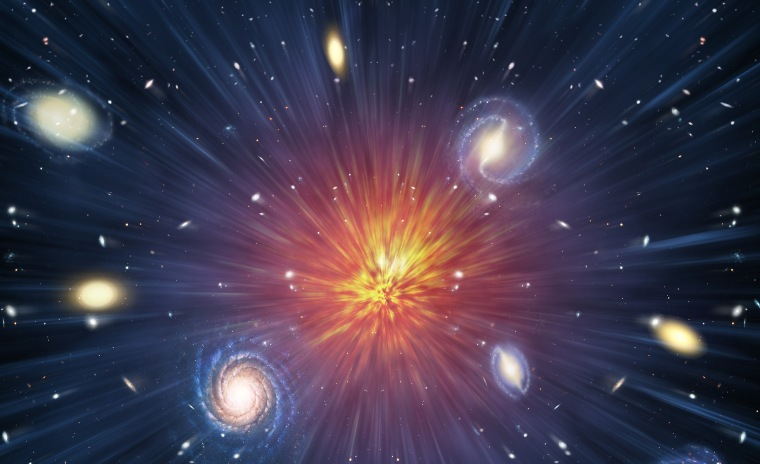
\includegraphics[width=2in]{universe.jpg}
    \caption{Figure Caption}
    \label{fig:my_label}
\end{figure}





\section{URL}
URL:       \url{https://sraf.nd.edu/}\\
Hyperlink: \hyperref[subsec:one]{Subsection One}\\
Weblink:   \href{https://www.google.com}{Google}\\





\section{Footnote}
Adding a footnote is as easy as writing your text\footnote{and then suddenly put everything inside \texttt{\textbackslash footnote\{\}}} and then continue writing where you left!


\newpage
\section{Sub Figures}
\begin{figure}[ht]

\begin{subfigure}{0.5\textwidth}
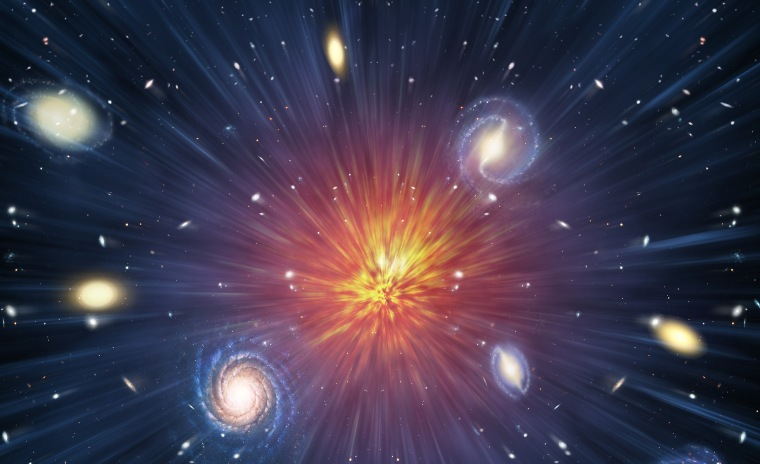
\includegraphics[width=0.9\linewidth]{universe.jpg} 
\caption{Sub-caption 1}
\end{subfigure}
% there should be no gap here!
\begin{subfigure}{0.5\textwidth}
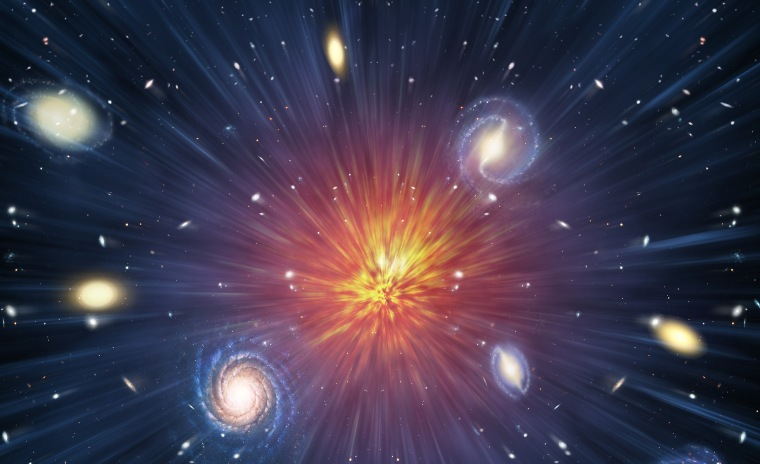
\includegraphics[width=0.9\linewidth]{universe.jpg}
\caption{Sub-caption 2}
\label{fig:subim2}
\end{subfigure}

\caption{Main caption}
\end{figure}




\section{parbox and Minipage}

\subsection{parbox}
\parbox{0.4\textwidth}{\raggedright \blindtext[1]} % raggedright justifies left
% no gaps here
\hspace{0.2\textwidth}
% no gaps here
\parbox{0.4\textwidth}{\raggedleft \blindtext[1]} % raggedleft justifies right

\subsection{Minipage}
\begin{minipage}{0.45\textwidth}
\blindtext[1]
\end{minipage}
% no space in between
\hspace{0.1\textwidth} % horizontal space between 2 minipages
\begin{minipage}{0.45\textwidth}
\blindtext[1]
\end{minipage}

\vspace{11pt} % vertical space between two minipages

\hspace{0.1\textwidth} % horizontal space before 3rd minipage
\begin{minipage}{0.8\textwidth}
\blindtext[1]
\end{minipage}
\hspace{0.1\textwidth} % horizontal space after 3rd minipage






\section{Math Symbols}
At any point in your test you can insert math by enclosing math formulas inside `\verb|$ $|` or `\verb|\( \)|`. You can math on a new line if you enclose math symbols within `\verb|\[ \]|' or `\verb|$$ $$|'.

Quadratic equation is $ax^2 + bx + c = 0$ with \( a > 0 \). The roots are given by \[ \frac{-b \pm \sqrt{b^2 - 4ac}}{2a} \]

Figure \ref{fig:math-symbols} gives a list of math symbols.

\begin{figure}[ht]
\centering
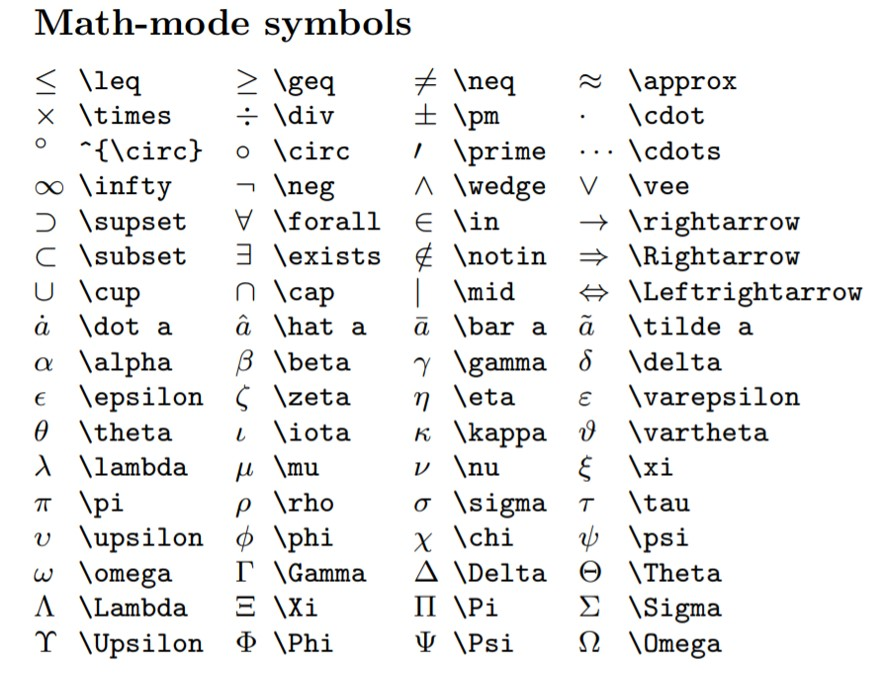
\includegraphics[width=6in]{math-symbols.jpg}
\caption{List of math symbols. There are many more. See \url{https://ctan.um.ac.ir/info/symbols/comprehensive/symbols-a4.pdf\#page=123}}
\label{fig:math-symbols}
\end{figure}






\newpage
\section{Equation}

See equation \ref{eq:diff}, 

\begin{equation}
    \frac{df}{dt} = \lim_{h \to 0} \frac{f(x+h) - f(x)}{h}
    \label{eq:diff}
\end{equation}

\begin{equation*}
    F = G \frac{m_1 m_2}{r^2}
\end{equation*}

% begin{equation*} is similar to $$ … $$ or \[ … \]

\begin{flalign}
\nonumber (x+y)^2 & = (x+y)(x+y) \\
\nonumber         & = x^2 +xy + yx + y^2 \\
\nonumber         & = x^2 +2xy + y^2
\end{flalign}

\begin{flalign}
&& (x+y)^2 & = (x+y)(x+y) \\
&&         & = x^2 +xy + yx + y^2 \\
&&         & = x^2 +2xy + y^2
\end{flalign}

\begin{flalign}
\nonumber (x+y)^2 & = (x+y)(x+y) && \\
\nonumber         & = x^2 +xy + yx + y^2 && \\
                  & = x^2 +2xy + y^2 &&
\end{flalign}





\section{Matrix}
\[
\begin{matrix}   \leq    &  \geq     \\  \neq      &  \cong       \end{matrix}   \hspace{2em}
\begin{pmatrix}  \infty  &  \lim     \\  \forall   &  \exists     \end{pmatrix}  \hspace{2em}
\begin{bmatrix}  \int    &  \iint    \\  \oint     &  \sum        \end{bmatrix}  \hspace{2em}
\begin{Bmatrix}  \oplus  &  \otimes  \\  \circ     &  \subset     \end{Bmatrix}  \hspace{2em}
\begin{vmatrix}  1/2     &  a^2      \\  \sqrt{5}  &  a_{22}      \end{vmatrix}  \hspace{2em}
\]





\section{Multi-page Table}
\begin{longtable}[t]{lccc} 

\caption{\label{tab:mytab}Disagreement by Industry}\\

\multicolumn{4}{p{\linewidth}}{
    \underline{\textbf{Optional Description}}: \blindtext[1]
}\\

\toprule

\textbf{Industry}                                                & 
\textbf{\% Sample}                                               & 
\textbf{\shortstack{Avg. Disagreement \\ (Ranks)}}               & 
\textbf{\shortstack{Std. Dev. of \\ Disagreement \\ (Ranks)}}   \\

\midrule
\endfirsthead

\caption*{Disagreement by Industry \textit{(continued)}}\\
\toprule

\endhead

\multicolumn{4}{p{\linewidth}}{
    \centerline{\textit{to be continued...}}
}

\endfoot

\bottomrule
\multicolumn{4}{p{\linewidth}}{
    \textit{Note:} \tableinfo
}

\endlastfoot


\textbf{Coal}      &  0.19  &  53.2  &  24.4  \\
Pharmaceuticals    &  5.52  &  69.6  &  22.3  \\
Precious-Metals    &  0.28  &  59.9  &  23.9  \\
Medical-Equipment  &  2.88  &  58.1  &  25.8  \\
Computers          &  3.43  &  56.2  &  24.9  \\
Real-Estate        &  0.75  &  56.0  &  24.6  \\
IT Services        &  9.87  &  54.3  &  24.9  \\
Construction       &  1.27  &  53.4  &  24.3  \\

\textbf{Coal}      &  0.19  &  53.2  &  24.4  \\
Pharmaceuticals    &  5.52  &  69.6  &  22.3  \\
Precious-Metals    &  0.28  &  59.9  &  23.9  \\
Medical-Equipment  &  2.88  &  58.1  &  25.8  \\
Computers          &  3.43  &  56.2  &  24.9  \\
Real-Estate        &  0.75  &  56.0  &  24.6  \\
IT Services        &  9.87  &  54.3  &  24.9  \\
Construction       &  1.27  &  53.4  &  24.3  \\

\textbf{Coal}      &  0.19  &  53.2  &  24.4  \\
Pharmaceuticals    &  5.52  &  69.6  &  22.3  \\
Precious-Metals    &  0.28  &  59.9  &  23.9  \\
Medical-Equipment  &  2.88  &  58.1  &  25.8  \\
Computers          &  3.43  &  56.2  &  24.9  \\
Real-Estate        &  0.75  &  56.0  &  24.6  \\
IT Services        &  9.87  &  54.3  &  24.9  \\
Construction       &  1.27  &  53.4  &  24.3  \\

\textbf{Coal}      &  0.19  &  53.2  &  24.4  \\
Pharmaceuticals    &  5.52  &  69.6  &  22.3  \\
Precious-Metals    &  0.28  &  59.9  &  23.9  \\
Medical-Equipment  &  2.88  &  58.1  &  25.8  \\
Computers          &  3.43  &  56.2  &  24.9  \\
Real-Estate        &  0.75  &  56.0  &  24.6  \\
IT Services        &  9.87  &  54.3  &  24.9  \\
Construction       &  1.27  &  53.4  &  24.3  \\

\textbf{Coal}      &  0.19  &  53.2  &  24.4  \\
Pharmaceuticals    &  5.52  &  69.6  &  22.3  \\
Precious-Metals    &  0.28  &  59.9  &  23.9  \\
Medical-Equipment  &  2.88  &  58.1  &  25.8  \\
Computers          &  3.43  &  56.2  &  24.9  \\
Real-Estate        &  0.75  &  56.0  &  24.6  \\
IT Services        &  9.87  &  54.3  &  24.9  \\
Construction       &  1.27  &  53.4  &  24.3  \\

\textbf{Coal}      &  0.19  &  53.2  &  24.4  \\
Pharmaceuticals    &  5.52  &  69.6  &  22.3  \\
Precious-Metals    &  0.28  &  59.9  &  23.9  \\
Medical-Equipment  &  2.88  &  58.1  &  25.8  \\
Computers          &  3.43  &  56.2  &  24.9  \\
Real-Estate        &  0.75  &  56.0  &  24.6  \\
IT Services        &  9.87  &  54.3  &  24.9  \\
Construction       &  1.27  &  53.4  &  24.3  \\

\textbf{Coal}      &  0.19  &  53.2  &  24.4  \\
Pharmaceuticals    &  5.52  &  69.6  &  22.3  \\
Precious-Metals    &  0.28  &  59.9  &  23.9  \\
Medical-Equipment  &  2.88  &  58.1  &  25.8  \\
Computers          &  3.43  &  56.2  &  24.9  \\
Real-Estate        &  0.75  &  56.0  &  24.6  \\
IT Services        &  9.87  &  54.3  &  24.9  \\
Construction       &  1.27  &  53.4  &  24.3  \\

\textbf{Coal}      &  0.19  &  53.2  &  24.4  \\
Pharmaceuticals    &  5.52  &  69.6  &  22.3  \\
Precious-Metals    &  0.28  &  59.9  &  23.9  \\
Medical-Equipment  &  2.88  &  58.1  &  25.8  \\
Computers          &  3.43  &  56.2  &  24.9  \\
Real-Estate        &  0.75  &  56.0  &  24.6  \\
IT Services        &  9.87  &  54.3  &  24.9  \\
Construction       &  1.27  &  53.4  &  24.3  \\

\end{longtable}





\section{Citing}
It is no surprise that the year 1905 is hailed as the miracle year of science. In a series of four papers Einstein (\citeyear{einstein1905_photo_electric, einstein_brownian, einstein_spc_rel, einstein_emc2}) changed the way we understand modern physics. \cite{einstein1905_photo_electric} demonstrated particle nature of light, \cite{einstein_brownian} gave evidence of existence of atoms, \cite{einstein_spc_rel} proposed modifications to notion of time at speeds approaching $c$ and \cite{einstein_emc2} finally showed equivalence between mass and energy through $E=mc^2$. Later, \cite{einstein_gen_rel} explained gravity as a curvature of spacetime against the accepted notion of it being a perceived force.

The first citation \cite{example} always list all authors. Subsequent citations \cite{example} will be abbreviated with `\verb|et al.|'. To get a full citation \cite*{example} use `\verb|\cite*|' instead.


\bibliography{references}


\end{document}
